% Latex template: mahmoud.s.fahmy@students.kasralainy.edu.eg
% For more details: https://www.sharelatex.com/learn/Beamer

\documentclass[aspectratio=1610]{beamer}					% Document class

\setbeamertemplate{footline}[text line]{%
  \parbox{\linewidth}{\vspace*{-8pt}A brief introduction to graphical models and deep methods in computational network biology \hfill\insertshortauthor\hfill\insertpagenumber}}
\setbeamertemplate{navigation symbols}{}

\usepackage[english]{babel}				% Set language
\usepackage[utf8x]{inputenc}			% Set encoding

\mode<presentation>						% Set options
{
  \usetheme{default}					% Set theme
  \usecolortheme{default} 				% Set colors
  \usefonttheme{default}  				% Set font theme
  \setbeamertemplate{caption}[numbered]	% Set caption to be numbered
}

% Uncomment this to have the outline at the beginning of each section highlighted.
%\AtBeginSection[]
%{
%  \begin{frame}{Outline}
%    \tableofcontents[currentsection]
%  \end{frame}
%}

\usepackage{graphicx}					% For including figures
\usepackage{booktabs}					% For table rules
\usepackage{hyperref}					% For cross-referencing
\usepackage[absolute,overlay]{textpos}
\usepackage{bm}

\title{Dynamics on gene networks}	% Presentation title
\author{Clayton W. Seitz}								% Presentation author
\date{\today}									% Today's date	

\begin{document}

% Title page
% This page includes the informations defined earlier including title, author/s, affiliation/s and the date
\begin{frame}
  \titlepage
\end{frame}

% Outline
% This page includes the outline (Table of content) of the presentation. All sections and subsections will appear in the outline by default.
\begin{frame}{Outline}
  \tableofcontents
\end{frame}

% The following is the most frequently used slide types in beamer
% The slide structure is as follows:
%
%\begin{frame}{<slide-title>}
%	<content>
%\end{frame}

\section{Introduction to biological networks}

\begin{frame}{Computational network biology}

Emerging research field that encompasses theory and applications of \textcolor{red}{network models} to study complex interactions of cells, DNA, RNA, proteins, and metabolites\\
\vspace{0.2in}
Say we have a set of variables $\bm{x} = (x_{1},x_{2},...,x_{n})$ which might have some statistical dependence. $\bm{x}$ might be RNA or protein expression data, for example\\
\vspace{0.2in}
\begin{itemize}
\item Often we are handed a batch of empirical samples $\bm{X} = \{\bm{x_{1}},..,\bm{x_{k}}\}$
\item We want to learn about the generating distribution $P(\bm{x},t)$
\end{itemize}

\vspace{0.2in}
Joint effort between physics, computer science, and biology

\begin{textblock*}{3cm}(12.25cm,5.5cm)
\begin{figure}
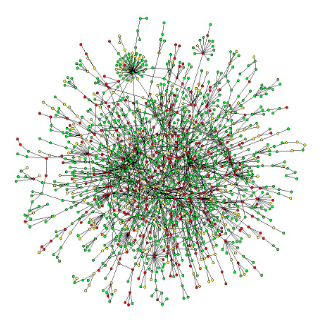
\includegraphics[width=3cm]{net.png}
\end{figure}
\end{textblock*}

\end{frame}

\begin{frame}{A gene interaction network}
\begin{center}
\begin{textblock*}{13cm}(1.3cm,1.5cm)
\begin{figure}
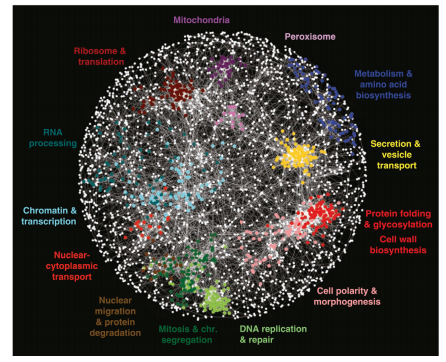
\includegraphics[width=8cm]{gene-network.png}
\caption{\textbf{Landscape of genetic interactions} in cells. Edges between genes denote Pearson correlation coefficients ($\rho > 0.2$) calculated from the
complete genetic interaction matrix.}
\end{figure}
\end{textblock*}
\end{center}
\end{frame}


\begin{frame}{Example gene regulatory network in yeast}

\begin{figure}
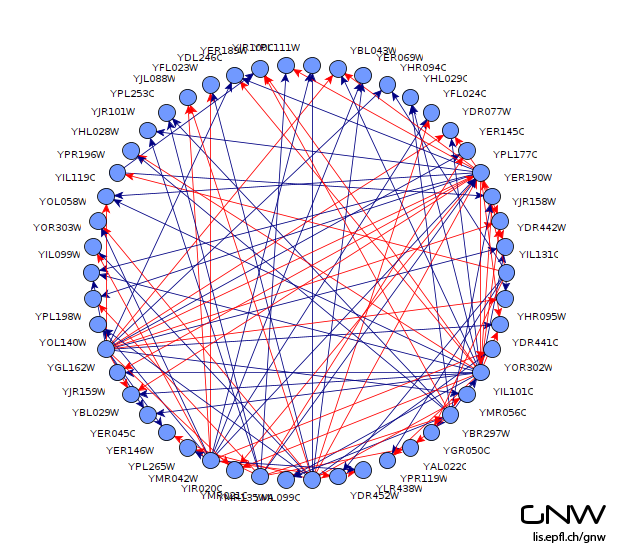
\includegraphics[width=9.5cm]{yeast-net.png}
\end{figure}

\end{frame}

\begin{frame}{Experimental considerations}

Gene interactions are inferred from gene expression data. RNA-seq has single cell-specificity and time resolution but lacks spatial resolution and data is noisy\\
\vspace{0.2in}
FISH techniques have single-cell specificity, spatial resolution, less noisy, but multiplexing is difficult\\
\vspace{0.2in}

High cost of multiplexing precludes acquisition of time-resolved data is single cell studies, which is important when statistics of the genes of interest are not stationary (circadian rhythms, cell-cycle, drug-treatment.\\
\vspace{0.2in}
Even when we can collect single-cell time-series data, data collected at a time point will contain extra variability due to asynchrony of cells within a population (in terms of progression through a biological process)\\

\end{frame}

\begin{frame}{Network modeling is hierarchical}

Fine structure of molecular interactions sometimes can be resolved for low dimensionality\\
\vspace{0.2in}
\textcolor{red}{Computational complexity} often scales exponentially with an increase in variables, density of interactions\\
\vspace{0.2in}
In high-dimensional biological networks we often turn to classic dimensionality reduction or hidden variable models\\


\end{frame}

\begin{frame}{Important topics}

Models range from networks of a few genes with detailed dynamical models to very large networks with coarse statistical description.
\vspace{0.2in}

\begin{itemize}
\item Linear dynamics of small networks (deterministic, stochastic)
\item Nonlinear dynamics of small networks (deterministic, stochastic) - Bintu model
\item Inferring network structure - Phi-Mixing Coefficient
\item Inferring network structure from linear dynamics - Hidden Markov Models
\item Inferring nonlinear network structure from empirical data - ?
\item Simulating stochastic dynamics (Gillespie algorithm)
\item Simulating stochastic nonlinear dynamics (Michaelis-Menten kinetics, SERGIO)
\end{itemize}


\end{frame}

\begin{frame}{Linear dynamics of transcription and translation}

\begin{textblock*}{15cm}(1cm,1.25cm)
Assumptions: gene-gene interactions are linear, noise is Gaussian, long protein lifetimes
\end{textblock*}

\begin{textblock*}{7cm}(0cm,1.75cm)
\begin{figure}
\begin{align*}
\dot{x_{i}} &= \sum_{j}m_{ij}y_{j} - \alpha_{i}x_{i} + \eta_{i}\\
\dot{y_{i}} &= r_{i}x_{i} - \beta_{i}y_{i}
\end{align*}
\end{figure}
\end{textblock*}

\begin{textblock*}{7cm}(1cm,4.75cm)
If we assume that $\dot{y_{i}} \approx 0$ we have a Langevin equation for $x(t)$ and \\$y/x = \beta/r$
\end{textblock*}

\begin{textblock*}{7cm}(7cm,1.75cm)
\begin{figure}
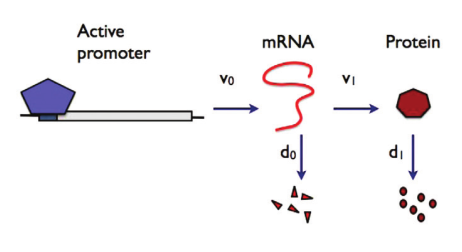
\includegraphics[width=7cm]{linear.png}
\end{figure}
\end{textblock*}

\begin{textblock*}{15cm}(1cm,6.5cm)

Let $\gamma_{ij} = m_{ij}\beta/r$. An example of a 3-gene system:

\begin{equation*}
\begin{bmatrix} 
    \dot{x_{1}}\\
	\dot{x_{2}}\\
	\dot{x_{3}}\\
    \end{bmatrix}
    =
\begin{bmatrix} 
    -\alpha_{1} & \gamma_{21} & \gamma_{31} \\
	\gamma_{12} & -\alpha_{2} & \gamma_{32}\\
	\gamma_{13} & \gamma_{23} & -\alpha_{3} \\
\end{bmatrix}
\begin{bmatrix} 
    x_{1}\\
	x_{2}\\
	x_{3}\\
    \end{bmatrix}
+ 
\begin{bmatrix} 
    \eta_{1}\\
	\eta_{2}\\
	\eta_{3}\\
    \end{bmatrix}
\end{equation*}

\end{textblock*}

\end{frame}

\begin{frame}{Ornstein-Uhlenbeck process}

We have a linear SDE, 

\begin{align*}
dx_{i} = \gamma_{ij}x_{j}dt + \sigma_{ij}dW
\end{align*}

which has a corresponding Fokker-Planck equation:

\begin{align}
\frac{\partial \tilde{P}(\vec{x},t)}{\partial t}= -\bm{\gamma_{ij}}\frac{\partial}{\partial x_{j}} x_{i}\tilde{P}(\vec{x},t) + D_{ij}\frac{\partial^{2} \tilde{P}(\vec{x},t)}{\partial x_{i}x_{j}}
\end{align}

If the real part of the eigenvalues of $\gamma_{ij}$ are greater than zero, a stationary distribution exists

\end{frame}

\begin{frame}{Conditional distributions of a Gaussian}

Partition variables $\{x_{n}\}_{n=1}^{N}$ into sets $\bm{x}_{a}$ and $\bm{x}_{b}$. 

\begin{align*}
\mu = \begin{bmatrix} 
    \mu_{a}\\
	\mu_{b}\\
    \end{bmatrix}
\;\;\;\;
\Sigma = \begin{bmatrix} 
    \Sigma_{aa} & \Sigma_{ab}\\
    \Sigma_{ba} & \Sigma_{bb}\\
    \end{bmatrix}
\end{align*}

The conditional distribution $p(\bm{x}_{a}|\bm{x}_{b})$ must also be normal with parameters

\begin{align*}
\mu_{a|b} &= \mu_{a} + \Sigma_{ab}\Sigma_{bb}^{-1}(x_{b}-\mu_{b})\\
\Sigma_{a|b} &= \Sigma_{aa}-\Sigma_{ab}\Sigma_{bb}^{-1}\Sigma_{ba}
\end{align*}

Bayesian networks loosely express causal relationships. We can compare $p(\bm{x}_{a}|\bm{x}_{b})$ and $p(\bm{x}_{a})$. \textcolor{red}{We can use this to assess quality of inference algorithms estimating the underlying network structure parameterized by the damping matrix} $\Gamma_{ij}$

\end{frame}

\begin{frame}{Marginal distributions of a Gaussian}

The conditional distribution $p(x_{1}|x_{2})$ between two variables $\bm{a}=x_{1}$, $\bm{b}=x_{2}$ has parameters

\begin{align*}
\mu_{1} &= \mu_{1} + \Sigma_{12}\Sigma_{22}^{-1}(x_{2}-\mu_{2})\\
\sigma_{1|2}^{2} &= \sigma_{1}^{2} -\Sigma_{12}\Sigma_{22}^{-1}\Sigma_{21}
\end{align*}

The multivariate normal has the nice property that marginal distributions are

\begin{align*}
p(x_{1}) &= \mathcal{N}\left(\mu_{1},\sigma_{1}^{2}\right)
\end{align*}

Conditional independence implies that $\mathcal{N}\left(\mu_{1},\sigma_{1}^{2}\right) = \mathcal{N}\left(\mu_{1|2},\sigma_{1|2}^{2}\right)$. We can then factor $p(\bm{x})$ into a Bayesian network. \\


\end{frame}

\begin{frame}{A scalable algorithm for inferring gene regulatory networks}

Interest in reverse-engineering whole-genome interaction networks from simultaneous measurements of the
expression levels of all (or at least most) genes in many
samples, under a common set of experimental conditions\\
\vspace{0.2in}
This algorithm applies when it is valid to assume that the system is in a steady state. For systems out of equilibrium, we need inference algorithms designed to operate on time-series data\\
\vspace{0.2in}
Typically gene expression data have low sampling rates and relatively small
amount of data. Moreover, GRNs have a high number of genes
with complex, nonlinear regulatory mechanisms

\end{frame}


\begin{frame}{The Phi-Mixing Coefficient}

Interest in reverse-engineering whole-genome interaction networks from simultaneous measurements of the
expression levels of all (or at least most) genes in many
samples, under a common set of experimental conditions\\
\vspace{0.2in}
This algorithm applies when it is valid to assume that the system is in a steady state. For systems out of equilibrium, we need inference algorithms designed to operate on time-series data\\
\vspace{0.2in}
Typically gene expression data have low sampling rates and relatively small
amount of data. Moreover, GRNs have a high number of genes
with complex, nonlinear regulatory mechanisms

\end{frame}

\section{References}

% Adding the option 'allowframebreaks' allows the contents of the slide to be expanded in more than one slide.
\begin{frame}[allowframebreaks]{References}
	\tiny\bibliography{references}
	\bibliographystyle{apalike}
\end{frame}

\end{document}
